\chapter{Experiments: Squeezed Light}
This chapter will cover the experimental methods used in the development of frequency-dependent squeezing in optomechanical systems, focusing on the generation of squeezed light, optical locking techniques, and quadrature measurement methods. The methods are designed to enhance the sensitivity of measurements in quantum optics and optomechanics.
\minitoc
\newpage 

\section{Optical Setup}

We first provide a general overview of the optical setup used to generate and manipulate squeezed light. 
Two lasers are used in this setup, to give flexibility as to produce bright squeezing directly from the OPO (one laser only), or produce vacuum squeezing to be mixed with a bright coherent field (two lasers). Both lasers are 1064nm Nd:YAG lasers (Coherent Mephisto and Mephisto S) as in the previous chapter. The full optical layout is shown in figure \ref{fig:opticallayout}. The experiment was designed as to easily switch between the two configurations. Throughout this chapter, we will refer to three different optical cavities common to the two configurations: the infrared mode cleaner (IRMC) cavity, the SHG cavity, and the OPO cavity. Each of these cavities is central to the generation and manipulation of squeezed light, and their characterization is detailed in the following sections. 

To generate bright squeezed light from an OPO, there are two configurations. The first one uses a single laser source, where the main laser beam is split into two paths. One path is directed to the SHG cavity to generate the second harmonic pump beam at 532nm, while the other path serves both for the Homodyne LO, as well as to seed the OPO with a bright field to be parametrically amplified or deamplified. 

The second configuration employs two independent lasers: one dedicated to pumping the SHG cavity and generating the 532nm pump beam, and the other serving as the LO for homodyne detection. This dual-laser setup allows for greater flexibility in controlling the relative phase and frequency between the pump and LO beams, which is crucial for optimizing squeezing measurements.


\section{Cavity Resonances and Locks}

\subsection{IRMC Cavity}
The first cavity presented here is the infrared mode cleaner (IRMC) cavity. The purpose of this cavity is to spatially filter the laser beam, ensuring a high-quality TEM00 mode profile, as well as \textit{cleaning} the IR beam from classical noise as developped in Chapter ??. 


\begin{figure}[h!]
    \centering  
    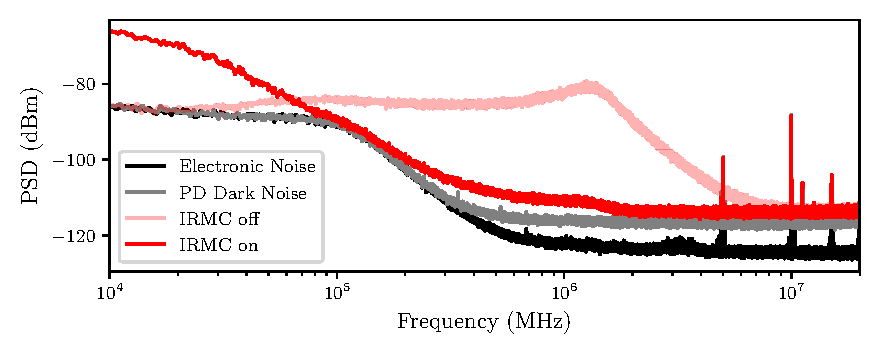
\includegraphics[width=\textwidth]{./chap6/fig/NoiseIRMC.pdf}
    \caption{}
    \label{fig:irmcnoise}
\end{figure}

\begin{figure}[h!]
    \centering  
    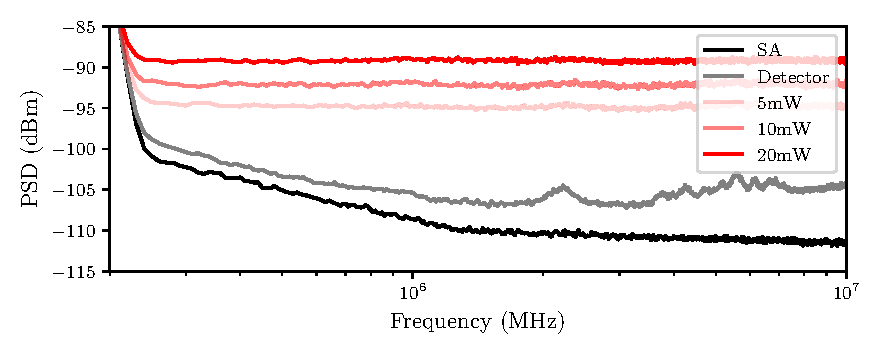
\includegraphics[width=\textwidth]{./chap6/fig/NoiseLO.pdf}
    \caption{}
    \label{fig:irmcnoise}
\end{figure}


\subsection{SHG Cavity}

In order to generate a stable $532\,\mathrm{nm}$ pump beam for the OPO, we implemented and characterized a linear SHG cavity. The cavity is designed to resonantly enhance an incoming IR field at $1064\,\mathrm{nm}$ and convert it into its second harmonic through a periodically poled lithium niobate (PPLN) crystal. In what follows we detail the characterization sequence.

\paragraph{Cavity Scanning and Resonance Mapping.}
The cavity is linear, with a length of $45 \, \text{mm}$, where both mirrors have a radius of curvature of $250 \, \text{mm}$: $L<2R$ so the cavity is stable. The input coupler has a transmission of $10 \%$ at $1064 \, \text{nm}$ and less than $1 \%$ at $532 \, \text{nm}$. The end mirror has a reflectivity of $99.9 \%$ for both $1064 \, \text{nm}$ and $532 \, \text{nm}$. This results in a theoretical cavity finesse of approximately $60$ at $1064 \, \text{nm}$, while the finesse at $532 \, \text{nm}$ would be around $1$, as no cavity buildup is desired at this wavelength.
Initial characterization was performed by scanning the cavity length around resonance using a piezoelectric transducer on which the cavity output coupler was glued. The input infrared power was maintained at approximately $100\,\mathrm{mW}$. The transmitted infrared signal and the generated green output were simultaneously monitored on fast photodiodes, while the PZT drive voltage was recorded to provide a calibrated frequency axis. 

Typical traces of the transmitted IR beam are shown in Fig.~\ref{fig:VL1}(b)–(c). As the cavity length is swept, the cavity exhibits sharp IR resonance peaks, corresponding to successive TEM00 modes of the cavity. At the same time, the green output rises only in coincidence with infrared resonances, confirming that efficient SHG occurs exclusively under resonant build-up of the fundamental field. The actual IR finesse was measured to be $\mathcal{F} = 35 \pm 0.6$, where the discrepancy is attributed to poor knowledge of the mirror parameters, as well as optical losses from the non linear medium. The polarization of the input beam is controled by half and quarter waveplates as to maximize the output green power, and the symmetry of the resonance peaks in the scans further indicates negligible birefringence in the PPLN crystal.


\paragraph{Cavity Locking.}
While scanning is useful for diagnostics, stable operation of the OPO pump requires continuous locking of the cavity to resonance. To achieve this, we employed a dither lock technique. The infrared input beam was phase-modulated at $\Omega_\mathrm{mod} = 19\,\mathrm{MHz}$ using a free space EOM (Photline NIR-MPX-LN-10). The transmitted infrared beam is demodulated and provides an error signal suitable for feedback to the PZT actuator. The cabling of the RedPitaya and other elements are detailed in Chapter ??.


\paragraph{Nonlinear Crystal and Phase Matching.}
The nonlinear medium is a commercially available PPLN chip from Covesion, with dimensions $10\times10\times1\,\mathrm{mm}^3$ and five parallel poling periods. Each grating corresponds to a different quasi-phase-matching period, enabling SHG for pump wavelengths near $1064\,\mathrm{nm}$ across a wide temperature range. For our Nd:YAG source we selected the $\Lambda \simeq 6.9\,\mu\mathrm{m}$ grating, designed for SHG around $65^{\circ}\mathrm{C}$. The crystal is AR coated at both $1064\,\mathrm{nm}$ and $532\,\mathrm{nm}$, limiting intra-cavity facet losses.

The conversion efficiency usually follows a sinc-squared dependence on temperature. Due to the high IR power build-up in the cavity, thermal effects are observed, which distort the expected sinc$^2$ shape as reported in ... When locking the cavity, hence stabilizing intracavity power at (relatively) high IR intensity, the non-linear crystal undergoes heating due to the IR absorption. Immediatly, its bulk starts to dillate, changing the quasi-phase matching conditions.  

After taking a rough quasi-phase matching curve not shown here, we identified the central peak and performed a fine scale scan of the crystal temperature at the IR input power allowing us to recover around $100$mW of green power, necessary to pump the OPO below threshold. For an input IR power of around $200$ mW, the generated green power as a function of temperature is shown in (a) of figure \ref{fig:shgtemp}, where we observed a tilt of the phase matching curve. The sinc$^2$ shape is however recovered when injecting an order of magnitude less IR power, but not useful to our purpose as it does not provide sufficient power for the OPO. The optimum is found at $58.37^{\circ}\mathrm{C}$ for the $6.90\,\mu\mathrm{m}$ grating, with a measured phase-matching bandwidth $\Delta T \simeq 1.5^{\circ}\mathrm{C}$ (FWHM). 

\paragraph{Temperature-Induced Resonance Shifts.}
In addition to determining phase-matching, the crystal temperature modifies the effective optical length of the cavity. As the temperature increases, the refractive index $n(T)$ rises, effectively lengthening the cavity. When the cavity is locked, an increase in intracavity IR power induces heating of the PPLN, which shifts the resonance condition. This thermal feedback manifests as a tilt in the transmission traces during PZT sweeps at high input powers [Fig.~\ref{fig:VL1}(c)]. 

At moderate powers ($P_\omega < 200\,\mathrm{mW}$) the effect is negligible, but at higher powers the thermo-optic shift dominates, causing a deviation from the ideal $\mathrm{sinc}^2$ dependence of the conversion efficiency. Instead, the efficiency curve skews and broadens, and thermal lensing within the crystal degrades the spatial overlap of the intracavity mode. In practice, we observed that beyond $\sim 200\,\mathrm{mW}$ of circulating IR power, the green output no longer increases linearly with $P_\omega$, but saturates due to these thermal effects.


\begin{figure}[h!]
    \centering  
    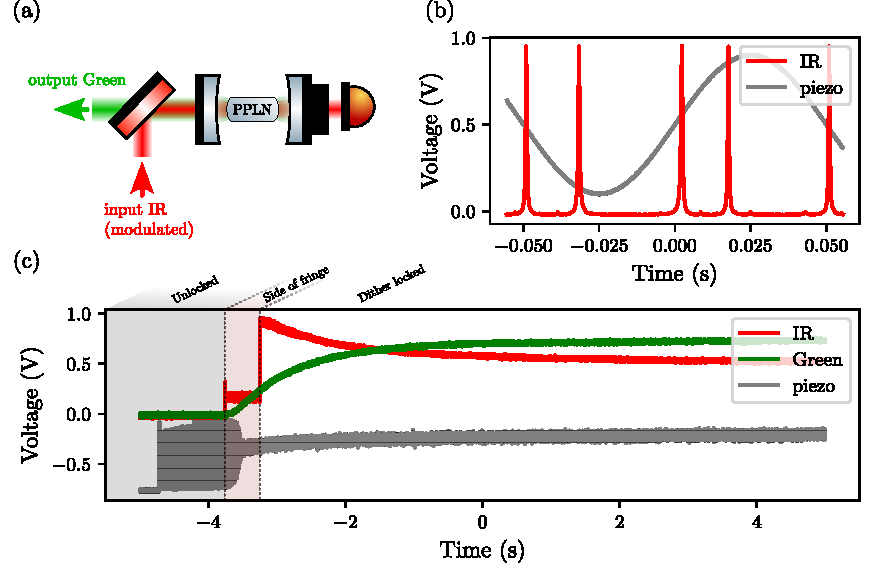
\includegraphics[width=\textwidth]{./chap6/fig/SHGlock_sweep.pdf}
    \caption{}
    \label{fig:shglock}
\end{figure}


\begin{figure}[h!]
    \centering  
    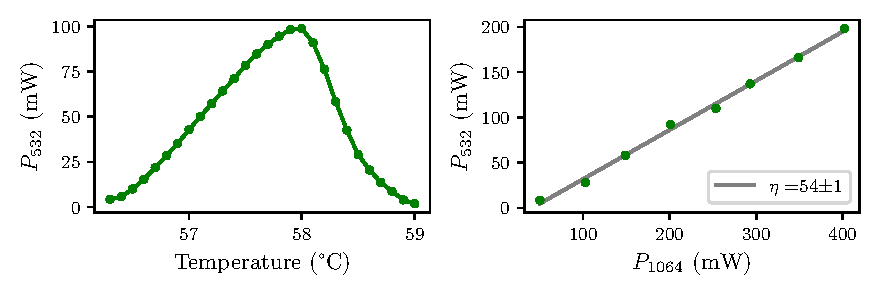
\includegraphics[width=\textwidth]{./chap6/fig/SHGscansTemp.pdf}
    \caption{}
    \label{fig:shgtemp}
\end{figure}



\subsection{OPO Cavity}

\section{Spectral analysis}
\subsection{Detection of Squeezing and Anti-squeezing}
\subsection{Spectral Variation with Frequency}
\subsection{Optimal Quadrature Conditions}
\section{Filter Cavity Concept}
\subsection{Virgo Filter Cavity }
\subsection{Thermal effects in bichromatic locks}